%        File: grundriss.tex
%     Created: Fr Jun 17 11:00  2016 Mitteleuropäische S
% Last Change: Fr Jun 17 11:00  2016 Mitteleuropäische S
%
\documentclass[border=10pt]{standalone}
\usepackage{pgfplots}
\usepackage{tikz}
\usetikzlibrary{shapes,positioning}

\tikzstyle{my dashed} = [dash pattern=on 10pt off 5pt]
\tikzstyle{my dashdotted} = [dash pattern=on 5pt off 2pt on \the\pgflinewidth off 2pt]
\begin{document}

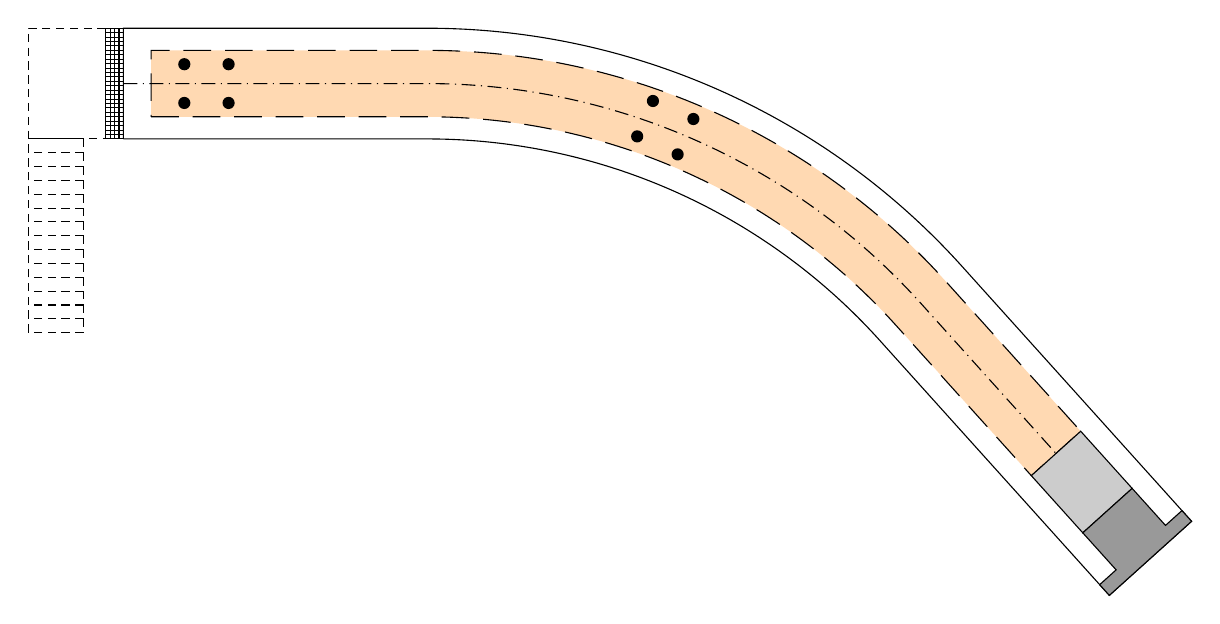
\begin{tikzpicture}[scale=0.2]
  \draw (0,0) -- ++(549pt,0) arc[radius=1100pt,start angle=90, end angle=42] -- ++(-48:620pt) coordinate (f1);
  \draw (0,0) -- (0,200pt) -- ++(549pt,0) arc[radius=1300pt,start angle=90, end angle=42] -- ++(-48:620pt) coordinate (f2) -- (f1);
  % Träger
  \draw[my dashed, fill=orange!30] (50pt,40pt) -- ++(499pt,0) arc[radius=1140pt,start angle=90, end angle=42] -- ++(-48:365pt) coordinate (b2) -- ++(42:120pt) coordinate (b1) -- ++(132:365pt) arc[radius=1260pt,start angle=42, end angle=90] -- ++(-499pt,0) -- cycle;
  % Central axis
  \draw[my dashdotted] (0,100pt) -- ++(549pt,0) arc[radius=1200pt,start angle=90, end angle=69] coordinate (m1) arc[radius=1200pt,start angle=69, end angle=42] -- ++(-48:620pt);
  % Beton
  \draw[fill=black!20] (b1) ++(-48:139pt) coordinate (b3) -- (b1) -- (b2) -- ++(-48:139pt) coordinate (b4) -- cycle;
  \draw[fill=black!40] (b3) ++(-48:90pt) -- (b3) -- (b4) -- ++(-48:90pt) -- ++(-138:40pt) -- (f1) -- (f2) -- ++(132:26pt) -- cycle;
  % Supports
  \draw (m1) ++(-24:40pt) ++(66:35pt) coordinate (p1);
  \draw (m1) ++(-24:40pt) ++(-114:35pt) coordinate (p2);
  \draw (m1) ++(156:40pt) ++(66:35pt) coordinate (p3);
  \draw (m1) ++(156:40pt) ++(-114:35pt) coordinate (p4);
  \fill[black] (p1) circle[radius=11pt];
  \fill[black] (p2) circle[radius=11pt];
  \fill[black] (p3) circle[radius=11pt];
  \fill[black] (p4) circle[radius=11pt];
  % Supports
  \coordinate (m2) at (150pt,100pt);
  \draw (m2) ++(0:40pt) ++(90:35pt) coordinate (p5);
  \draw (m2) ++(0:40pt) ++(-90:35pt) coordinate (p6);
  \draw (m2) ++(180:40pt) ++(90:35pt) coordinate (p7);
  \draw (m2) ++(180:40pt) ++(-90:35pt) coordinate (p8);
  \fill[black] (p5) circle[radius=11pt];
  \fill[black] (p6) circle[radius=11pt];
  \fill[black] (p7) circle[radius=11pt];
  \fill[black] (p8) circle[radius=11pt];
  % Treppe
  \draw[densely dashed] (-32pt,0) -- ++(0,200pt) -- ++(-140pt,0) -- ++(0,-200pt) -- cycle;
  \draw[densely dashed] (-72pt,0) -- ++(0,-350pt) -- ++(-100pt,0pt) -- ++(0pt,350pt) -- cycle;
  \foreach \step in {1,...,13}{
    \draw[densely dashed] (-72pt, -\step*350pt / 14) -- ++(-100pt,0);
  }
  %
  \foreach \ix in {0,8,16,...,200}{
    \draw[] (0pt,\ix *1pt) -- ++(-32pt,0);
  }
  \foreach \iy in {0,8,16,...,32}{
    \draw[] (\iy *-1pt, 0) -- ++(0,200pt);
  }
\end{tikzpicture}


\end{document}


